\documentclass{beamer}
\setbeamertemplate{itemsize items}{ball}
\usepackage[utf8]{inputenc}
\usepackage[T1]{fontenc}
\usepackage{lmodern}
\usepackage{graphicx}
\usetheme{Singapore}

\begin{document}
    \titlegraphic{
\includegraphics[width=4.2cm]{2000px-Fub-logo.png}}
	\author{Presented by: Dhruti Lalaji Sawant}
	\institute {Freie Universität Berlin - Institut für Informatik 	\vspace{3pt} Seminar on Internet of Things and Security (Seminar Technische Informatik)}
	\title{Securing IoT Networking with ICN}
   	\date{13th November, 2018}
	\setbeamercovered{transparent}
	\setbeamertemplate{navigation symbols}{}
\begin{frame}[plain]
\maketitle
\end{frame}

\begin{frame}
\frametitle{Overview}
\begin{itemize}
	\item Introduction
	\item Related work in the area IoT networking
	\item Structure of the report
	\item List of References
	\item Tentative schedule
	\item Open Questions
\end{itemize}
\end{frame}	

\begin{frame}
\frametitle{Introduction}
\begin{itemize}
	\item The TCP/IP\footnote{Transmission Control Protocol/Internet Protocol} model did not include security and privacy abstractions in its initial design in the early 1980s
	\item Thus creating several layer extensions to existing protocols and data overheads  in todays applications to provide secure functionalities
\end{itemize}
 
\begin{figure}
	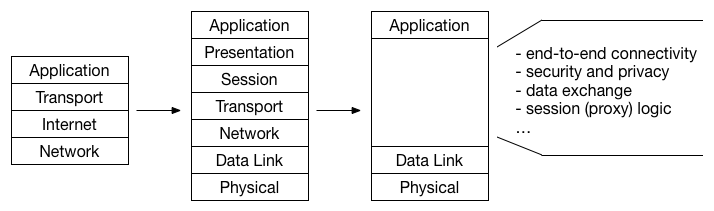
\includegraphics[width=\linewidth,height=0.3\textheight]{ccn_stack.png}
	\caption{TCP/IP Layers and its functionalities.}
\end{figure}


\end{frame}
\begin{frame}
\frametitle{Introduction}
\begin{itemize}
	\item ICN\footnote{Information-Centric Networking}offers an alternative to networking in a secure and private manner that reduces the technical overhead of TCP/IP model
	\item It focuses on transmitting and accessing named content instead of the traditional host-based IP data
\end{itemize}
 

\begin{figure}
	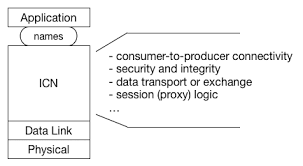
\includegraphics[width=0.6\linewidth,height=0.4\textheight]{stack.png}
	\caption{ICN Stack layers.}
\end{figure}
\end{frame}

\begin{frame}
\frametitle{Related work in the area IoT networking}
\begin{itemize}
	\item Security improvement in IoT based on Software
	Defined Networking (SDN)


	\item The virtus middleware: An xmpp based architecture for secure iot communications
\end{itemize}

\end{frame}
\begin{frame}
\frametitle{Structure of the report}
\begin{itemize}
	\item[1.]Introduction \\
	The ICN protocol stack will be introduced.
	\item[2.]Networking in IoT \\
	The ICN middleware architecture will be explained in detail.
	\item[3.]Secure Functionalities\\
	The services provided by this architecture withh be explained.
	\item[4.]Discussion\\
	The topic will be further discussed.
	\item[5.]Conclusion\\
	The conclusion will be drawn.
\end{itemize}
\end{frame}
\begin{frame}
\frametitle{List of References}
\begin{itemize}
	\item[1.]\href {https://ieeexplore.ieee.org/document/7962667}{A Secure ICN-IoT Architecture} 
	\item[2.]\href {http://conferences2.sigcomm.org/acm-icn/2017/files/tutorial-ndn-ccnlite-riot/2-Why-ICN-for-IoT.pdf}{Why IoT with ICN?}
	\item[3.]\href{http://delivery.acm.org/10.1145/3080000/3079070/p425-Conti.pdf}{Do we need a holistic approach for the design of secure IoT
		systems?}
	\item[4.] \href {http:delivery.acm.org/10.1145/2670000/2660144/p77-baccelli.pdf?}{Information centric networking in the IoT: experiments with NDN in the wild}
\end{itemize}
	
\end{frame}
\begin{frame}
\frametitle{Tentative schedule}
\begin{itemize}
	\item By 18.11.2018: Section Networking in IoT
	\item By 30.11.2018: Section Secure functionalities 
	\item By 09.12.2018: Sections Discussion and Conclusion
	\item By 16.12.2018: Revise and improvements
\end{itemize}
\end{frame}
\begin{frame}
Thank you for your attention.
\end{frame}
\end{document}
